\documentclass[danish, a4paper, onecolumn, oneside]{article}

\usepackage{preamble}
\usepackage[document]{ragged2e} % Align text til venstre
% EDIT PATH
%\graphicspath\left\{ ./Graphics/}}

% Indkommentere nedenstående, hvis der skal indsættes kode
%\usepackage{minted}
\usepackage{csquotes}



\pretitle{\begin{center}\Huge\bfseries}
\title{A WKB-Type Approximation to the Schrödinger Equation}
\posttitle{\par\vskip1em{\normalfont\normalsize\scshape  Projektstiller: Philip Daniel Blocher,
\\ Instruktor: Philip Daniel Blocher,
\\ Department of Physics and Astronomy
\\ - Fælles besvarelse \par\vfill}\end{center}}
\author{%
        René Czepluch(StudNr)       \thanks{rene.czepluch@post.au.dk},
   \and Rasmus Klitgaard(StudNr)    \thanks{rasmusklitgaard97@gmail.com},
   \and Laurits N. Stokholm(StudNr) \thanks{laurits.stokholm@post.au.dk}

   }

\predate{\vfill\begin{center}\large}

%\institute{Department of Physics and Astronomy}
   \date{\today}

   %\usepackage[backend=biber, style=authortitle, defernumbers=true, sorting=nty]{biblatex}
   %\addbibresource{bib.bib}
%
\begin{document}
\begin{titlingpage}
\maketitle
\end{titlingpage}
\noindent
%TODO SØRG FOR TEKSTØRRRELSEN ER 11 PT
\section{Indledning}

\section{Solution to the stationary Schrödinger Equation}

Antages, at der betragtes en partikel i en dimension, $x$,  er Schrödinger ligningen
%
\begin{equation}
    \frac{\hbar^2}{2m}\frac{\partial^2 \psi}{\partial x^2} + V(x) \psi = E \psi
    \label{eq:scrodingerLigning1}
\end{equation}
%
isoleres $\frac{\partial^2 \psi}{\partial x^2}$ i \cref{eq:scrodingerLigning1}, opnås

\begin{equation}
    \frac{\partial^2 \psi}{\partial x^2} = 2m\psi (E  - V(x)) \frac{1}{\hbar^2}
    \label{eq:scrodingerLigning2}
\end{equation}

defineres $p(x)$ klassisk

\begin{equation}
p(x) \equiv \sqrt{2m(E-V(x))}
\end{equation}
Kan \cref{eq:scrodingerLigning2} omskrives til

\begin{equation}
    \frac{\partial^2 \psi}{\partial x^2} = - \frac{p(x)^2}{\hbar^2} \psi.
    \label{eq:scrodingerLigning3}
\end{equation}

Anvendes ansatzen

\begin{equation}
    \psi(x) = A(x) e^{i \phi(x)}
    \label{eq:ansatz}
\end{equation}

hvor $\psi (x) \in \mathbb{C}$. Antages

\begin{equation}
 E > V(x) \forall x
\end{equation}

Er $A(x)$ en reel amplitude og $\phi(x)$ er en reel fase. Dette kan altid gøres, der man ved hjælp af ledet  $e^{i \phi(x)} $. Dette led danner en vektor $ \in \mathbb{C}$ med normen 1. Herefter kan $A(x)$  skalere vektoren, til at ramme alle punkter. Anvendes venstre side af \cref{eq:scrodingerLigning3} på \cref{eq:ansatz} fås

\begin{equation}
    \frac{\partial \psi}{\partial x} = \left(i A{\left (x \right )} \frac{d}{d x} \phi{\left (x \right )} + \frac{d}{d x} A{\left (x \right )}\right) e^{i \phi{\left (x \right )}}
    \label{eq:diff1gange}
\end{equation}

\begin{align}
    \frac{\partial^2 \psi}{\partial x^2} = \left(- A{\left (x \right )} \left(\frac{d}{d x} \phi{\left (x \right )}\right)^{2} + i A{\left (x \right )} \frac{d^{2}}{d x^{2}}  \phi{\left (x \right )} + 2 i \frac{d}{d x} A{\left (x \right )} \frac{d}{d x} \phi{\left (x \right )} + \frac{d^{2}}{d x^{2}}  A{\left (x \right )}\right) e^{i \phi{\left (x \right )}}
    \label{eq:diff2gange}
\end{align}

Dette må også være lig med højre side af \cref{eq:scrodingerLigning3}. Substitueres udtrykket for $\psi$ fra \cref{eq:ansatz} kan \cref{eq:diff2gange} reduceres til

\begin{align}
    \left(- A{\left (x \right )} \left(\frac{d}{d x} \phi{\left (x \right )}\right)^{2} + i A{\left (x \right )} \frac{d^{2}}{d x^{2}}  \phi{\left (x \right )} + 2 i \frac{d}{d x} A{\left (x \right )} \frac{d}{d x} \phi{\left (x \right )} + \frac{d^{2}}{d x^{2}}  A{\left (x \right )}\right) e^{i \phi{\left (x \right )}} = - \frac{p^2}{\hbar^2} \psi = - \frac{p(x)^2}{\hbar^2} A(x) e^{i \phi(x)}
    \label{eq:udskrevet}
\end{align}

\begin{equation}
     \Rightarrow - A{\left(x \right)} \left(\frac{d}{d x} \phi{\left(x \right)}\right)^{2} + i A{\left(x \right)} \frac{d^{2}}{d x^{2}}  \phi{\left(x \right)} + 2 i \frac{d}{d x} A{\left(x \right)} \frac{d}{d x} \phi{\left (x \right )} + \frac{d^{2}}{d x^{2}}  A{\left (x \right )}
     = - \frac{p(x)^2}{\hbar^2} A(x)
     \label{eq:ReOgIm}
\end{equation}

Sorteres venstre side af \cref{eq:ReOgIm} real delen og imaginær delen fås henholdsvis

\begin{equation}
    A{\left (x \right )} \left(\frac{d}{d x} \phi{\left (x \right )}\right)^{2}  + \frac{d^{2}}{d x^{2}}  A{\left (x \right )}
    = - \frac{p(x)^2}{\hbar^2} A(x)
    \label{eq:Re}
\end{equation}

\begin{equation}
    i A{\left (x \right )} \frac{d^{2}}{d x^{2}}  \phi{\left (x \right )} + 2 i \frac{d}{d x} A{\left (x \right )} \frac{d}{d x} \phi{\left (x \right )}
    = - \frac{p(x)^2}{\hbar^2} A(x)
    \label{eq:Im}
\end{equation}

Af disse kan\cref{eq:Im}  løses, løsningen er: % er det rigtigt? Hvorfor er der ingen løsning i Realdelen

\begin{equation}
    A(x) = \frac{C}{\sqrt{(\frac{d}{d x} \phi{\left (x \right )})}}.
    \label{eq:ImLoes}
\end{equation}

Hvor C er en konstant. Der eksisterer ingen løsninger til \cref{eq:Re}, og derfor foretages en approximation, ved blot at droppe $\frac{d^{2}}{d x^{2}}  A{\left (x \right )}$ leddet i samme ligning. Dette er en god approixmation, hvis $A(x)$ varier langsomt. Da kan \cref{eq:Re} omskrives til

\begin{equation}
    \left(\frac{d}{d x} \phi{\left (x \right )}\right)^{2}
    = - \frac{p(x)^2}{\hbar^2}
    \label{eq:ReApprox}
\end{equation}

\begin{equation}
    \Rightarrow \frac{d}{d x} \phi{\left (x \right )}
    = \pm \frac{p(x)}{\hbar}
    \label{eq:ReApproxFinal}
\end{equation}

Integreres med hensyn til x på begge sider, opnås

\begin{equation}
    \phi(x) = \pm \frac{1}{\hbar} \int p(x) dx.
    \label{eq:daPhi}
\end{equation}



\begin{equation}
    \psi(x) \cong \frac{C}{\sqrt{p(x)}} e^{\phi(x)} \cong \frac{C}{\sqrt{p(x)}} e^{\pm \frac{1}{\hbar} \int p(x) dx}
    \label{eq:final}
\end{equation}

\section{Potentialebrønd med vertikale vægge}
Lad os betragte det klassiske system, $E > V(x) \ \forall x \in[a,b]$, hvor intervallet $[a,b]$ er det begrænsede interval med $a$ og $b$ som klassiske vendepunkter. Heri eksisterer bølgefunktionen $\psi(x)$, ækvivalent til en brønd med vertikale vægge. Lad $|\psi(a)|^{2} = 0 = |\psi(b)|^{2}$. Fra \cref{eqpsi} vil man kunne skrive $\psi(x)$ som en sum af hhv. negativ og positiv eksponent.

\begin{equation}
    \psi(x) \cong \frac{1}{\sqrt{p(x)}}\left[C_{+}e^{i\phi(x)}+C_{-}e^{-i\phi(x)}\right].
  \label{eq:kvantiseringStart}
\end{equation}
Ved at definere to nye konstanter, $C_1 \equiv i(C_{+}-C_{-})$ og $C_2 \equiv C_{+}+C_{-}$, kan dette ved brug af eulers identitet skrives om til
\begin{equation}
  \psi(x) = \frac{1}{\sqrt{p(x)}}
  \Bigl[    C_1\sin{\phi(x)} + C_2\cos{\phi(x)}   \Bigr].
  \label{eq:kvantiseringSinCos}
\end{equation}
Her gælder det, at $\phi(x) = \frac{1}{\hbar}\int p(x) dx$. Integreres over intervallet $[a, x]$, vil
\begin{equation}
  \phi(x) = \frac{1}{\hbar}\int_{a}^{x} p(x')dx'.
\end{equation}
Fra startbetingelsen kræves at $\psi(a) = 0 = \psi(b)$. Da\footnote{Dette kan nemt ses, ved at integrere fra og til $a$} $\phi(a) = 0$, må $C_2$ være 0, da $\cos(0)\neq 0$. Dette medfører at,
\begin{equation}
    \psi(x) = \frac{1}{\sqrt{p(x)}}C_1\sin{\phi(x)}.
\end{equation}
Nu skal det stadig gælde at $\psi(b) = 0$, og da $C_1\neq 0$\footnote{Dette er en ikke normerbar løsning, og en ret kedelig en af slagsen.}, må det altså betyde at $\sin(\phi(b)) = 0$, hvilket medfører at $\phi(b) = n'\pi$, hvor $n' = 0, 1, 2\ldots$.
Resultatet bliver
\begin{equation}
  \int_{a}^{b} p(x) dx = n'\pi\hbar
  \label{eq:kvantiDone}
\end{equation}

\section{Brintatomet}
Den radiale Schrödingerligningen er givet ved \cite[s. 140]{griffiths}
%
\begin{align}
    \frac{-\hbar^{2}}{2m}\diff[2]{u(r)}{r} + \left( - \frac{e^{2}}{4\pi\epsilon_{0}r} + \frac{\hbar^{2}}{2m}\frac{l(l+1)}{r^{2}} \right)u(r) & \nonumber = Eu(r)
    \label{eq:schroedinger3d}
\end{align}
%
hvor $V_{\text{eff}}$ er en sum af det velkendte Coulomb potentiale og et led tilhørende den ekstra, rotationelle frihedsgrad.

hvor $V_{\text{eff}}$ er en sum af Coulomb potentialet og et led tilhørende et angulært moment.

Fra \cite{griffiths} kendes bohrradien, $a_{0}$ og Rydbergenergien $\mathrm{Ry}$ til følgende værdier;

\begin{align}
    a_{0} = & \frac{\hbar^{2}}{2m}\left( \frac{e^{2}}{4\pi\epsilon_{0}} \right) \\
\mathrm{Ry} = & \frac{m}{2\hbar^{2}}\left( \frac{e^{2}}{4\pi\epsilon_0} \right)^{2}
\label{eq:konstanter}
\end{align}

Sættes energien til at være et multiplum af Rydbergenergien, $E = -\varepsilon \mathrm{Ry}$, og genkendes det, at $a_{0}^{2}\mathrm{Ry} = \frac{\hbar^{2}}{2m}$, samt at $2a_{0}\mathrm{Ry} = \frac{e^{2}}{4\pi\epsilon_{0}}$, kan \fxnote{reference} skrives
\begin{align}
    k(r) = & \frac{1}{\hbar} \sqrt{2m\left( E - V_{\text{eff}} \right)}\\
    = & \sqrt{\frac{1}{a_{0}^{2}\mathrm{\mathrm{Ry}}} \left( E + \frac{e^{2}}{4\pi\epsilon_{0}r} - \frac{\hbar^{2}}{2m}\frac{l(l+1)}{r^{2}} \right)}\\
    = & \sqrt{\frac{1}{a_{0}^{2}\mathrm{Ry}} \left( (-\varepsilon \mathrm{Ry}) + \frac{2a_{0}\mathrm{Ry}}{r} - a_{0}^{2}\mathrm{Ry}\frac{l(l+1)}{r^{2}} \right)}\\
    = & \frac{1}{r} \sqrt{\frac{1}{a_{0}^{2}{Ry}} \left( (-\varepsilon \mathrm{Ry})r^{2} + 2a_{0}\mathrm{Ry} r - a_{0}^{2}\mathrm{Ry} l(l+1) \right)}
\end{align}
Trækker vi her $\frac{1}{a_0}$ udenfor og ganger $\mathrm{Ry}$ ind i parantesen får vi
\begin{align}
  k(r) = & \frac{1}{a_0} \frac{1}{r} \sqrt{-\varepsilon r^2 + 2a_0r - a_0^2l(l+1)} \\
  = & \frac{\sqrt{\varepsilon}}{a_0} \frac{1}{r} \sqrt{r^2 - \frac{2a_0}{\varepsilon}r + \frac{a_0^2}{\varepsilon}l(l+1)}
\end{align}

Nu er det indre i kvadratroden på en form som kan skrives som noget $(x-a)(x-b) = x^2 -x(a+b) + ab$. Nu undersøges det om man kan ende ud med at få disse $a$ og $b$ størrelser til at være de klassiske vendepunkter, som er de $r$ som opfylder at $k(r) = 0$.
Da det udenfor kvadratroden i $k(r)$ ikke kan være 0, sættes det indre lig 0.
\begin{equation}
  r^2 - \frac{2a_0}{\varepsilon}r + \frac{a_0^2}{\varepsilon}l(l+1) = 0
\end{equation}
Dette har løsninger ved
\begin{align}
  r = & \frac{\frac{2a_0}{\varepsilon} \pm \sqrt{\frac{4a_0^2}{\varepsilon^2} - \frac{4a_0^2}{\varepsilon}l(l+1)   }  }{2}\\
    = & \frac{a_0}{\varepsilon}[1+\sqrt{1-\varepsilon l(l+1)}]
\end{align}
Herved bliver de klassiske vendepunkter
\begin{align}
  a =  \frac{a_0}{\varepsilon}\Bigl[1-\sqrt{1-\varepsilon l(l+1)}  \Bigr],\qquad b =  \frac{a_0}{\varepsilon}\Bigl[1+\sqrt{1-\varepsilon l(l+1)}  \Bigr]
\end{align}
For at det nu skal passe i vores udtryk for $k(r)$ tjekkes det om
\begin{align}
  a+b = & \frac{2a_0}{\varepsilon} \\
  ab  = & \frac{a_0^2}{\varepsilon} l(l+1)
\end{align}
$a+b$ leddet er oplagt, mens $ab$ leddet bliver
\begin{align}
  ab = & \frac{a_0^2}{\varepsilon^2}\Bigl(1-\sqrt{1-\varepsilon l(l+1)} \Bigr)\Bigl(1+\sqrt{1-\varepsilon l(l+1)} \Bigr)\\
     = & \frac{a_0^2}{\varepsilon^2}\Bigl(1-(1-\varepsilon l(l+1)) \Bigr) =  \frac{a_0^2}{\varepsilon^2} \varepsilon l(l+1)
     = \frac{a_0^2}{\varepsilon} l(l+1)
\end{align}

Det ses at det passer og derfor kan vi arbejde videre med disse værdier $a$ og $b$.
\begin{align}
  k(r) = & \frac{p(r)}{\hbar} = \frac{\sqrt{\varepsilon}}{a_0}\frac{1}{r}\sqrt{(r-a)(r-b)}
\end{align}
Nu kan vi altså integrere fra $a$ til $b$, som er de klassiske vendepunkter og bruge \cref{eq:kvantiDone}.
\begin{equation}
  \int_{a}^{b}k(r)dr = \frac{\sqrt{\varepsilon}}{a_0} \Bigl[\frac{\pi}{2}(\sqrt{b}-\sqrt{a})^2  \Bigr]
\end{equation}
Her er det brugt at
\begin{equation}
  \int_{\alpha}^{\beta}\frac{1}{u}\sqrt{(u-\alpha)(u-\beta)}du = \frac{\pi}{2}(\sqrt{\beta}-\sqrt{\alpha})^2
\end{equation}
Herfra følger det at
\begin{align}
  n' = & \frac{\sqrt{\varepsilon}}{2a_0}(\sqrt{b}-\sqrt{a})^2 = \frac{\sqrt{\varepsilon}}{2a_0}(b+a-2\sqrt{ab})\\
     = & \frac{\sqrt{\varepsilon}}{2a_0}\Bigl(\frac{2a_0}{\varepsilon}-2a_0\sqrt{\frac{1}{\varepsilon}l(l+1)}\Bigr)\\
     = & \frac{1}{\sqrt{\varepsilon}} -l(l+1)
\end{align}
Herfra finder vi $\varepsilon$ til at være
\begin{equation}
  \varepsilon = \frac{1}{\Bigl[n'+l(l+1)  \Bigr]^2}
\end{equation}
Og da $E = -\varepsilon Ry$, så kan vi skrives
\begin{equation}
  E_{n',l} = \frac{-Ry}{\Bigl[n'+l(l+1)  \Bigr]^2}
\end{equation}

Nu kigger vi på den asymptotiske form for bølgefunktionerne ved store $r$.
I det eksakte tilfælde er de på formen
\begin{equation}
  R_{nl}(r) \sim \left(\frac{r}{a_0}\right)^{n-1}e^{-r/na_0}
\end{equation}

For at finde dem i WKB tilfældet kigges først på formen af en sådan bølgefunktion. Det kan vises at den er på formen %TODO find formen her
\begin{equation}
  u(r) \sim exp\Bigl[-\int_{a_0}^{r}k(r')dr'\Bigr]
\end{equation}
Først kigges der på $k(r)$ da vi gerne vil lave en rækkeudvikling da vi kun kigger på meget store $r$.
Vi har altså at
\begin{equation}
  k(r) = \frac{\sqrt{\varepsilon}}{a_0}\frac{1}{r}\sqrt{(r-a)(r-b)}
\end{equation}
Her lader vi $\frac{1}{r}$ gå ind under kvadratroden og vi får
\begin{align}
  k(r) = & \frac{\sqrt{\varepsilon}}{a_0}\sqrt{(1-\frac{a}{r})(1-\frac{b}{r})} = \frac{\sqrt{\varepsilon}}{a_0}\sqrt{1-\frac{a+b}{r}+\frac{ab}{r^2}}
\end{align}
Her beholder vi kun til første orden og vi får altså noget som vi kan rækkeudvikle ved den sædvanelige kvadratrods række.
\begin{align}
  k(r) \approx & \frac{\sqrt{\varepsilon}}{a_0}\sqrt{1-\frac{a+b}{r}}\\
       = & \frac{\sqrt{\varepsilon}}{a_0}(1-\frac{1}{2}\frac{a+b}{r})
\end{align}
Husker vi på $a+b = \frac{2a_0}{\varepsilon}$ så får vi
\begin{equation}
  k(r) = \frac{\sqrt{\varepsilon}}{a_0}-\frac{1}{\sqrt{\varepsilon}r}
\end{equation}
\\
Kigger vi da på integralet har vi at
\begin{align}
  \int_{a_0}^{r}k(r')dr' = & \frac{\sqrt{\varepsilon}}{a_0}(r-a_0) - \frac{1}{\sqrt{\varepsilon}}\left(\ln{r}-\ln{a_0}\right)\\
  = & \frac{\sqrt{\varepsilon}}{a_0}(r-a_0) - \ln{((\frac{r}{a_0})^{\frac{1}{\sqrt{\varepsilon}}})}
\end{align}

Så nu kan vi altså skrive vores $u(r)$ op som
\begin{align}
  u(r) \sim & \exp\left[-\frac{\sqrt{\varepsilon}}{a_0}(r-a_0) + \ln{((\frac{r}{a_0})^{\frac{1}{\sqrt{\varepsilon}}})}\right]\\
        = & \exp\left[-\frac{\sqrt{\varepsilon}}{a_0}(r-a_0)\right] + (\frac{r}{a_0})^{\frac{1}{\sqrt{\varepsilon}}}\\
        = & \exp\left[\sqrt{\varepsilon}(1-\frac{r}{a_0})\right] + (\frac{r}{a_0})^{\frac{1}{\sqrt{\varepsilon}}}
\end{align}
Nu bruges det blot at
\begin{equation}
  \varepsilon = \frac{1}{\left[n'+\sqrt{l(l+1)}\right]^2}
\end{equation}
Og det giver os altså at
\begin{equation}
  u(r) \sim {\left(\frac{r}{a_0}\right)}^{\left[n'+\sqrt{l(l+1)}\right]} e^{\left[\frac{1-\frac{r}{a_0}}{n'+\sqrt{l(l+1)}}\right]}
\end{equation}

%TODO kommenter det her resultat og sammenlign
Dette giver os også at $R(r) = u(r)/r$ bliver
\begin{equation}
  R(r) = \frac{1}{a_0}{\left(\frac{r}{a_0}\right)}^{\left[n'-1+\sqrt{l(l+1)}\right]} e^{\left[\frac{1-\frac{r}{a_0}}{n'+\sqrt{l(l+1)}}\right]}
\end{equation}
Plottes $V_{\text{eff}}$

\begin{figure}[h!]
    \centering
    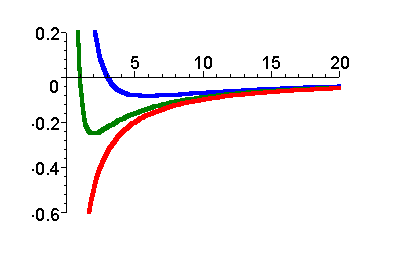
\includegraphics[width=\columnwidth]{hydrogen}
    \caption{Hydrogen}
    \label{fig:hydrogen}
\end{figure}


%
%%

\section{Solution to the stationary Schrödinger Equation}
\section{Tunnelering}

\section{Ionisation af et Rydberg-atom}

\section{Konklusion}
I denne rapport undersøges WKB approksimationen. Først udledes approksimationen fra Schrödingerligningen, i én dimension. Vi finder en løsning der bygger på at $V(x)$ varierer langsomt, i forhold til bølgelængden af $\psi(x)$, og dermed forventer at et mere konstant potentiale giver et bedre svar. Eksempelvis finder vi, at approksimationen faktisk levere et eksakt svar, til de tilladte energier for et uendeligt brøndpotentiale. Dernæst undersøges brintatomet. Vi finder at energiernes løsninger afhænger af kvantetallet $l$, og at WKB-approksimationen giver bedre resultater, når det gælder at $n'$ er meget større end $l$. Det ved vi, da vi netop kan løse energierne for brint eksakt. Afslutningsvist undersøges den asymptotiske form for bølgefunktionerne for brint hvor det findes at approksimationen går imod de eksakte løsninger for store radier $r$.




\end{document}
